\documentclass[a4paper]{article}\usepackage[]{graphicx}\usepackage[]{color}
%% maxwidth is the original width if it is less than linewidth
%% otherwise use linewidth (to make sure the graphics do not exceed the margin)
\makeatletter
\def\maxwidth{ %
  \ifdim\Gin@nat@width>\linewidth
    \linewidth
  \else
    \Gin@nat@width
  \fi
}
\makeatother

\definecolor{fgcolor}{rgb}{0.345, 0.345, 0.345}
\newcommand{\hlnum}[1]{\textcolor[rgb]{0.686,0.059,0.569}{#1}}%
\newcommand{\hlstr}[1]{\textcolor[rgb]{0.192,0.494,0.8}{#1}}%
\newcommand{\hlcom}[1]{\textcolor[rgb]{0.678,0.584,0.686}{\textit{#1}}}%
\newcommand{\hlopt}[1]{\textcolor[rgb]{0,0,0}{#1}}%
\newcommand{\hlstd}[1]{\textcolor[rgb]{0.345,0.345,0.345}{#1}}%
\newcommand{\hlkwa}[1]{\textcolor[rgb]{0.161,0.373,0.58}{\textbf{#1}}}%
\newcommand{\hlkwb}[1]{\textcolor[rgb]{0.69,0.353,0.396}{#1}}%
\newcommand{\hlkwc}[1]{\textcolor[rgb]{0.333,0.667,0.333}{#1}}%
\newcommand{\hlkwd}[1]{\textcolor[rgb]{0.737,0.353,0.396}{\textbf{#1}}}%
\let\hlipl\hlkwb

\usepackage{framed}
\makeatletter
\newenvironment{kframe}{%
 \def\at@end@of@kframe{}%
 \ifinner\ifhmode%
  \def\at@end@of@kframe{\end{minipage}}%
  \begin{minipage}{\columnwidth}%
 \fi\fi%
 \def\FrameCommand##1{\hskip\@totalleftmargin \hskip-\fboxsep
 \colorbox{shadecolor}{##1}\hskip-\fboxsep
     % There is no \\@totalrightmargin, so:
     \hskip-\linewidth \hskip-\@totalleftmargin \hskip\columnwidth}%
 \MakeFramed {\advance\hsize-\width
   \@totalleftmargin\z@ \linewidth\hsize
   \@setminipage}}%
 {\par\unskip\endMakeFramed%
 \at@end@of@kframe}
\makeatother

\definecolor{shadecolor}{rgb}{.97, .97, .97}
\definecolor{messagecolor}{rgb}{0, 0, 0}
\definecolor{warningcolor}{rgb}{1, 0, 1}
\definecolor{errorcolor}{rgb}{1, 0, 0}
\newenvironment{knitrout}{}{} % an empty environment to be redefined in TeX

\usepackage{alltt}

%% Language and font encodings
\usepackage[english]{babel}
\usepackage[utf8x]{luainputenc}
\usepackage[T1]{fontenc}

%% Sets page size and margins
\usepackage[a4paper,top=3cm,bottom=2cm,left=3cm,right=3cm,marginparwidth=1.75cm]{geometry}

%% Useful packages
\usepackage{amsmath,parskip,palatino, graphicx}
%\usepackage[colorinlistoftodos]{todonotes}
\usepackage[colorlinks=true, allcolors=blue]{hyperref}


\setlength\parindent{0em}


\title{M.S. Writing Project}
\author{Andrea Mack}
\IfFileExists{upquote.sty}{\usepackage{upquote}}{}
\begin{document}
\maketitle

%\begin{abstract}
%Your abstract.
%\end{abstract}

\section*{Schedule}

\begin{table}[h!]
\centering
\begin{tabular}{c|c}
Week of & Tasks \\\hline
Jan 23 & \begin{tabular}[t]{@{}c@{}}Review Ch.2 Banerjee, Carlin, \& Gelfand \\
Look at R software for simulating and fitting variograms. \end{tabular}  \\
\hline
Jan 30 & \begin{tabular}[t]{@{}c@{}} Simulate data with known covariance structure \\ Fit Bayesian spatial model to simulated data \\ Start annotated bibliography  \end{tabular}\\
\hline
Feb 6 & \\
Feb 13 & \\
Feb 20 & \\
Feb 27 & \\
Mar 6 & \\
Mar 13 & \\
Mar 20 & \\
Mar 27 & \\
Apr 3 & \\
Apr 10 & \\
Apr 17 & \\
Apr 24 & \\
Apr 31 & Writing Project Due:\\
\hline
\end{tabular}
\caption{\label{tab:schedule}Writing Project Schedule}
\end{table}


\section*{Package Exploration}

\subsection*{GeoR}


\section*{Future Research Ideas}
\begin{itemize}

\item Modeling how the SE moves through the lake; extensions to generally modeling how things move (blood flow through body, mineral deposits change in a mine, modeling tumor growth- somewhat inspired by Margaret's abstract)

\item

\end{itemize}



\section*{Annotated Bibliography}
\todo[inline, color=red!50]{Andy add more papers to this list}


\subsection*{Bayesian Geospatial Design, Peter Diggle and Soren Lophaven}
In \cite{diggle2006} the authors specify design criteria as the minimum posterior predictive variance for both prospective and retrospective designs. Univariate response case. 


\subsection*{An Introduction to Model-based Geostatistics}

The authors describe a method for calculating posterior predictive variance in both prospective and retrospectie case. \cite{diggle2003}

\subsection*{Optimal Spatio-temporal Hybrid Sampling Designs for Ecological Monitoring}

The authors in \cite{hooten2009} specified a method for optimal designs for dynamic spatial temporal processes. Dynamic is in the sense that the process changes over time. Compared designs for hybrid and fixed designs. Hybrid designs combine fixed sites to sample each year and random sites which vary each year. Fixed (static) sites are more convenient while dynamic sites show how the process changes over time and the ``inherent spatial autocorrelation". Criteria specified was the minumum average prediction variance. Favored sites have the most spatial variation and are least correlated with other sites (Wikle and Royle, 1999).

Process:
1) Leave out observation t and use all other observations to predict $y_{t}$. 

2) Compute $Var(Y_{t} | Y_{t-1,...1})$ for all t.

3) Average (2).

4) Retain minimum (3).

Method handles multivariate response model through $m_{t}$:

\begin{center}
${\bf Y_{t}} = {\bf K_{t}\alpha_{t}\Phi_{t}^{T}} + {\bf \epsilon_{t}\phi_{t}^{T}}$
\end{center}

${\bf Y_{t}}$ = $m_{t} X n$ multivariate response vector
${\bf K_{t}}$ = $m_{t} X n$ maps observations to process vector
{\bf $\alpha_{t}$} = true latent process
${\bf \Phi_{t}}$ = matrix to transform to univariate spatial observation

Criteria was using Kalman filtering. Benfits of Kalman filtering include allowing estimatation of latent process ({\bf $\alpha$}) as well as it's uncertainty. {\it check is this similar to incorproating bayes in diggle's paper to min estimation and pred. var?}

\vspace{1in}

{\bf Kalman filter reference} \url{http://www.cs.unc.edu/~welch/kalman/}

\section*{Heirarchial Modeling - Analysis for Spatial Data}

\subsection*{Chapter 2}

\begin{itemize}
\item {\bf Stationarity}: 

1) Strong - distribution constant over entire domain

2) Weak - $Cov(y_{t},y_{t+h})$ = C(h) - the covariance between two observations depends only on the separation vector between them, can also state that the mean is constant over the entire domain, but not necessary

3) Intrinsic - {\bf Semi-variogram} = $\gamma(h) = \frac{Var(y_{t} - y_{t+h})}{2}$ = $Var(y) + Cov(y_{t},y_{t+h})$ = c(0) + c(h) - the average variance between two observations depends only on the separation vector between them

\begin{itemize}

\item Gaussian response \rightarrow weak stationarity imples strong stationarity

\item Weak stationarity \rightarrow intrinsic stationarity

\item {\bf Ergodic} - if c(h) \rightarrow 0 as ||h|| \rightarrow \inf, then intrinsic stationarity \rightarrow weak stationarity

\item $\gamma(h)$ == {\bf Variogram}, and must be negative defninte

\end{itemize}

\item {\bf Isotrophic} - $\gamma(h)$ depends only on the separation vector through its length (vs. direction, etc.) - likely Benton Lake data are not isotrophic - {\it How to deal with this?}

\item {\bf Homogenous} = intrinsic + isotrophic

\item {\bf Semivariogram} - plot of the semivariogram vs. ||h||, can also have directional where multiple ``lines", one for each direction considered

\item Notation

\begin{itemize}
\item $\tau^{2}$ = nugget = ``non-spatial" variance component

\item $\sigma^{2}$ = partial sill = ``spatial" variance component

\item $\tau^{2} + \sigma^{2}$ = sill

\item $\gamma(h)$ = $\tau^{2} + \sigma^{2}$*Correlation Structrure

\item R = range = distance at which $\gamma(h)$ = $\tau^{2} + \sigma^{2}$, responses are no longer correlated

\item If R = \inf, then create {\bf effective range}

\end{itemize}

\end{itemize}

Options for choosing the correlation function:

\begin{enumerate}
\item Empirical compared to theoretical, but make sure valid - Gaussian, exponential, and cauchy always valid

\item Criteria penalizing complexity and rewarding parsimony

\item Theoretical foundations

\item Matern class

\end{enumerate}

{\bf The correlation structure informs smoothness.}

{\it Explain difference between intrinsic and weak stationarity.}

{\it Odd Matern $\tau^{2}$}


\newpage
\section*{Project Outline:}
\section{Introduction}

\section{Data}

% \section{Model}

\section{Simulation Studies}

\section{Results}

\section{Concluding Thoughts}

\newpage 
\section{Latex / Overleaf code}
\subsection{How to include Figures}

\begin{figure}[h!]
\centering
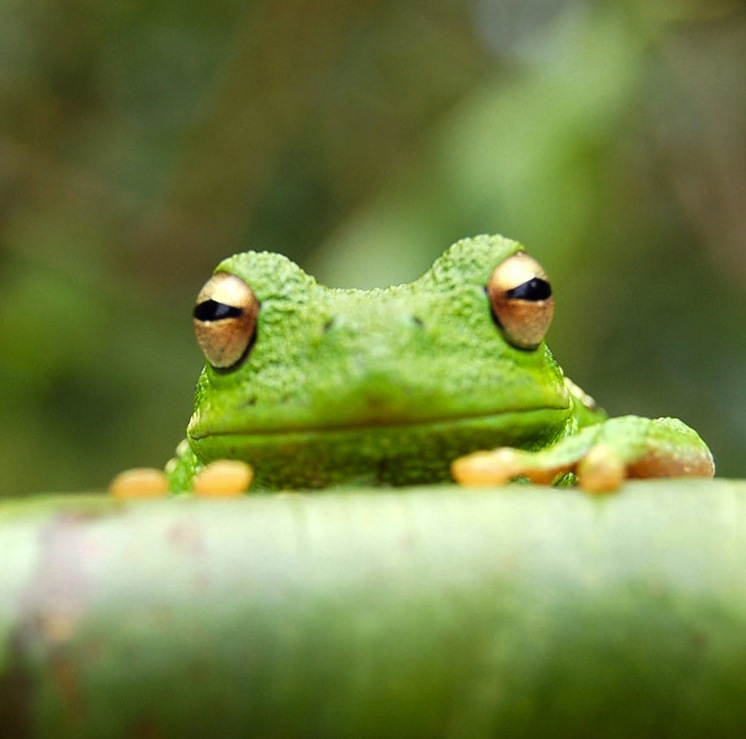
\includegraphics[width=0.3\textwidth]{frog.jpg}
\caption{\label{fig:frog}This frog was uploaded via the project menu.}
\end{figure}



First you have to upload the image file from your computer using the upload link the project menu. Then use the includegraphics command to include it in your document. Use the figure environment and the caption command to add a number and a caption to your figure. See the code for Figure \ref{fig:frog} in this section for an example.

\subsection{How to add Comments}

Comments can be added to your project by clicking on the comment icon in the toolbar above. % * <john.hammersley@gmail.com> 2016-07-03T09:54:16.211Z:
%
% Here's an example comment!
%
To reply to a comment, simply click the reply button in the lower right corner of the comment, and you can close them when you're done.

Comments can also be added to the margins of the compiled PDF using the todo command\todo{Here's a comment in the margin!}, as shown in the example on the right. You can also add inline comments:

\todo[inline, color=green!40]{This is an inline comment.}

\subsection{How to add Tables}

Use the table and tabular commands for basic tables --- see Table~\ref{tab:widgets}, for example. 

\begin{table}[h!]
\centering
\begin{tabular}{l|r}
Item & Quantity \\\hline
Widgets & 42 \\
Gadgets & 13
\end{tabular}
\caption{\label{tab:widgets}An example table.}
\end{table}



\bibliographystyle{apalike}
\bibliography{refsSpatial}

\end{document}
